\documentclass[aspectratio=169]{beamer}

\usepackage[utf8]{inputenc}
%\usepackage{latexsym}
\usepackage{graphicx}
\usepackage{mathptmx}
\usepackage{amsmath}
%\usepackage{amsfonts}
\usepackage{amssymb}
\usepackage{amsbsy}
\usepackage{amsthm}
\usepackage{algorithmic}
% \usepackage{subcaption}
\usepackage{tikz}
\usepackage[T1]{fontenc}

% Get checkmark logo
\usepackage{pifont}
\newcommand{\cmark}{\ding{51}}
\newcommand{\xmark}{\ding{55}}
% Get \lee and \gee commands
\newcommand{\lee}{\leqq}
\newcommand{\gee}{\geqq}

% Strikouts
\usepackage[normalem]{ulem}

% Restore Mathcal
\let\saveboldmath\boldmath
\usepackage{mathptmx}
\let\boldmath\saveboldmath
\usepackage{bm}
\DeclareSymbolFont{cmsymbols}{OMS}{cmsy}{m}{n}
\SetSymbolFont{cmsymbols}{bold}{OMS}{cmsy}{b}{n}
\DeclareSymbolFontAlphabet{\mathcal}{cmsymbols}

\usepackage[english]{babel}
\usepackage[utf8]{inputenc}

% AMSLaTeX packages
\usepackage{amsthm}
\usepackage{amsmath}
\usepackage{amsfonts}
\usepackage[algoruled]{algorithm2e}

\usetheme{default}
\useoutertheme{default}
% we want to use images
\usepackage{graphicx}
\usepackage{movie15}
\usepackage{hyperref}

% table relates packages
\usepackage{booktabs}
\usepackage{multirow}
% pick a font
\usepackage{palatino}           
% \usepackage{times}
\usepackage{tikz}
\usetikzlibrary[positioning,arrows,decorations.pathmorphing,backgrounds,fit,calc]
% \AtBeginSection[]  % "Beamer, do the following at the start of every section"
% {
%   \begin{frame}<beamer> 
%     \frametitle{Outline} % make a frame titled "Outline"
%     \tableofcontents[currentsection]  % show TOC and highlight current section
%   \end{frame}                    
% }

% \AtBeginSubsection[]
% {
%   \begin{frame}
%     \frametitle{Outline}
%     \tableofcontents[currentsection,currentsubsection]
%   \end{frame}
% }

\AtBeginSection[]
{
   \begin{frame}
       \frametitle{Outline}
       \tableofcontents[currentsection]
   \end{frame}
}

\newcommand{\ebox}[1][1em]{\framebox[#1]{\phantom{M}}}

\setlength\arraycolsep{1.4pt}% some length

%gets rid of navigation symbols
\setbeamertemplate{navigation symbols}{}

%gets rid of bottom navigation bars
\setbeamertemplate{footline}[page number]{}
\setbeamertemplate{headline}{}


\usebackgroundtemplate{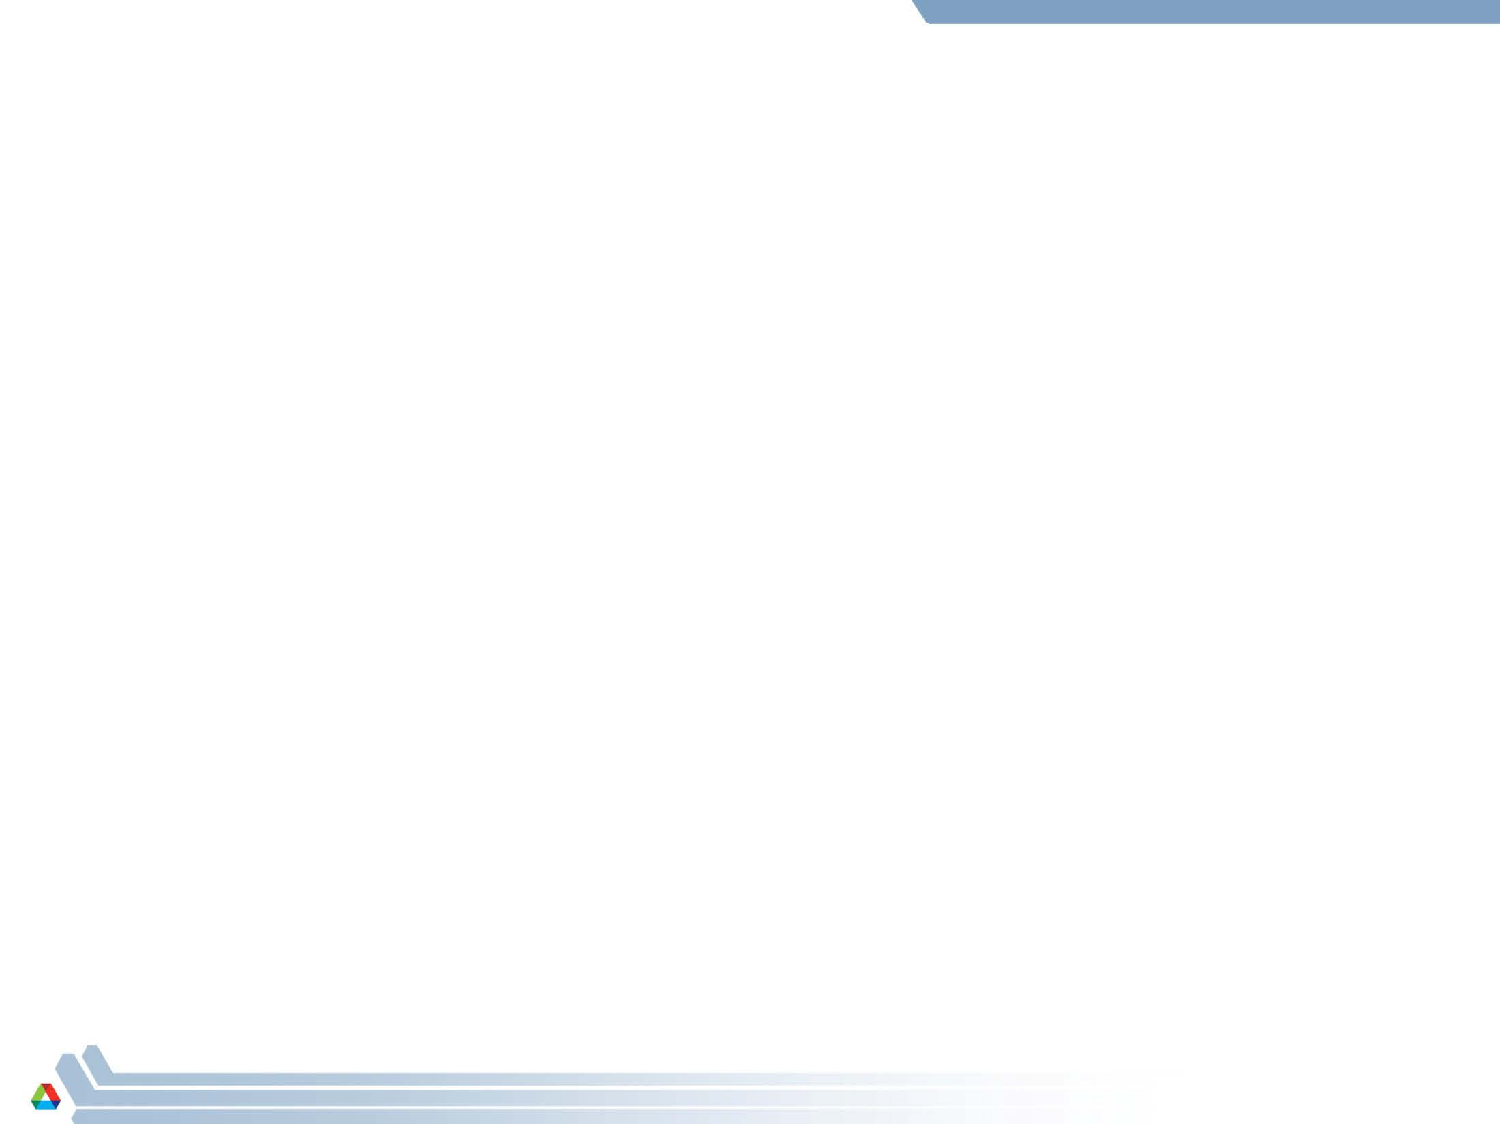
\includegraphics[width=\paperwidth]{../templates/NormalANLBlue}}

% Title Information
\title{
An Integrated Multi-Physics Optimization Framework for Particle Accelerator Design}

\author{Gongxiaohui Chen$^{a}$, Tyler Chang$^{a}$, John Power$^{a}$, and
    Chungunag Jing$^{b}$}
\date{WSC 2023, San Antonio, TX, USA\\
Dec XX, 2023}
\institute{$^a$Argonne National Laboratory, $^b$Euclid TechLabs}

\begin{document}

\setbeamertemplate{footline}{}
{
\usebackgroundtemplate{
\includegraphics[width=\paperwidth]{../templates/TitleANLBlue}}
\frame{\titlepage}
}

\setbeamertemplate{footline}[page number]{}

% FRAME: overview
\begin{frame}
  \frametitle{Outlines}
  \tableofcontents
\end{frame}

\section{Introduction to a simplified accelerating beamline}

\begin{frame}{Introduction to a simplified accelerating beamline}
\begin{columns}
% Column 1 
\begin{column}{0.6\textwidth}
    \begin{figure}
    \centering
        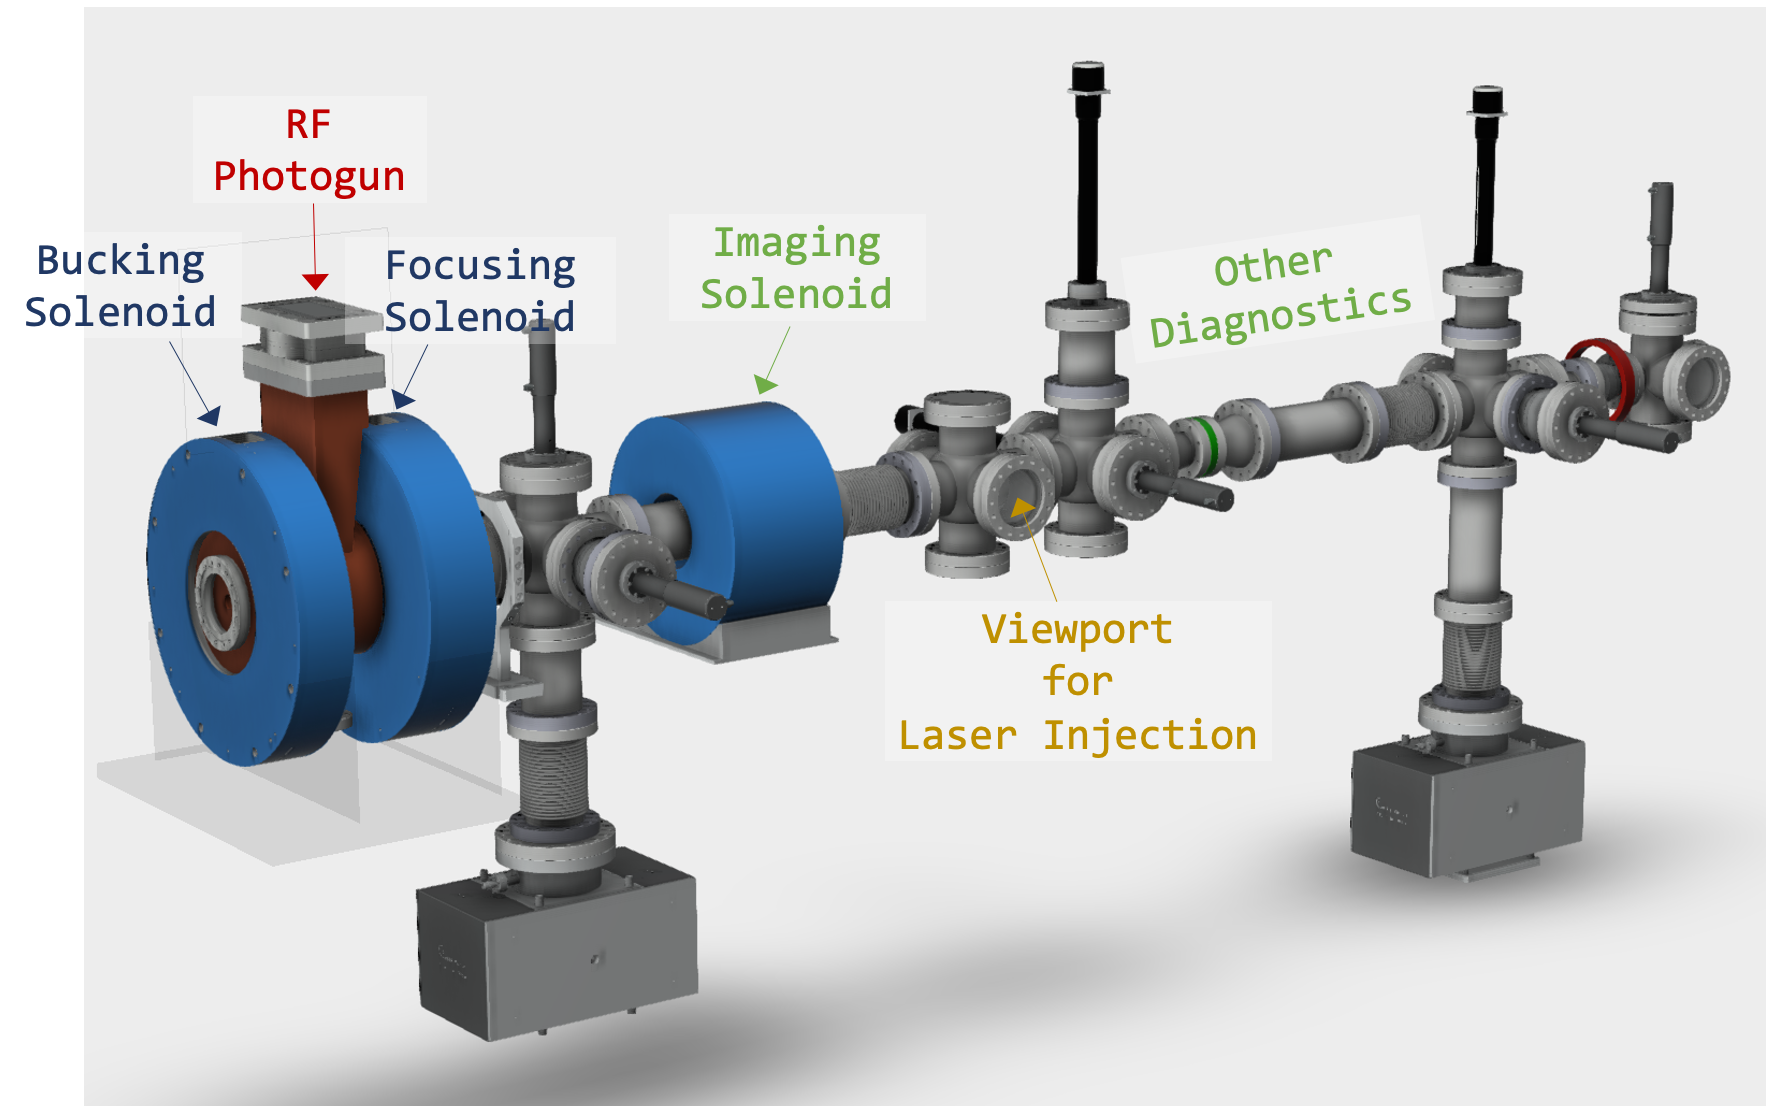
\includegraphics[width=1\textwidth]{beamline1_1.png}
    \end{figure}
\end{column}
% Column 2
\begin{column}{0.4\textwidth}
A standard accelerating beamline includes:
        \begin{itemize}
            \item RF photogun 
            \item Bucking/focusing solenoid (or main solenoid)
            \item Other magnets or diagnostics 
        \end{itemize}
\end{column}
\end{columns}
\end{frame}

\begin{frame}{Introduction to a RF photogun}
\begin{columns}
% Column 1 
\begin{column}{0.6\textwidth}
    \begin{figure}
    \centering
        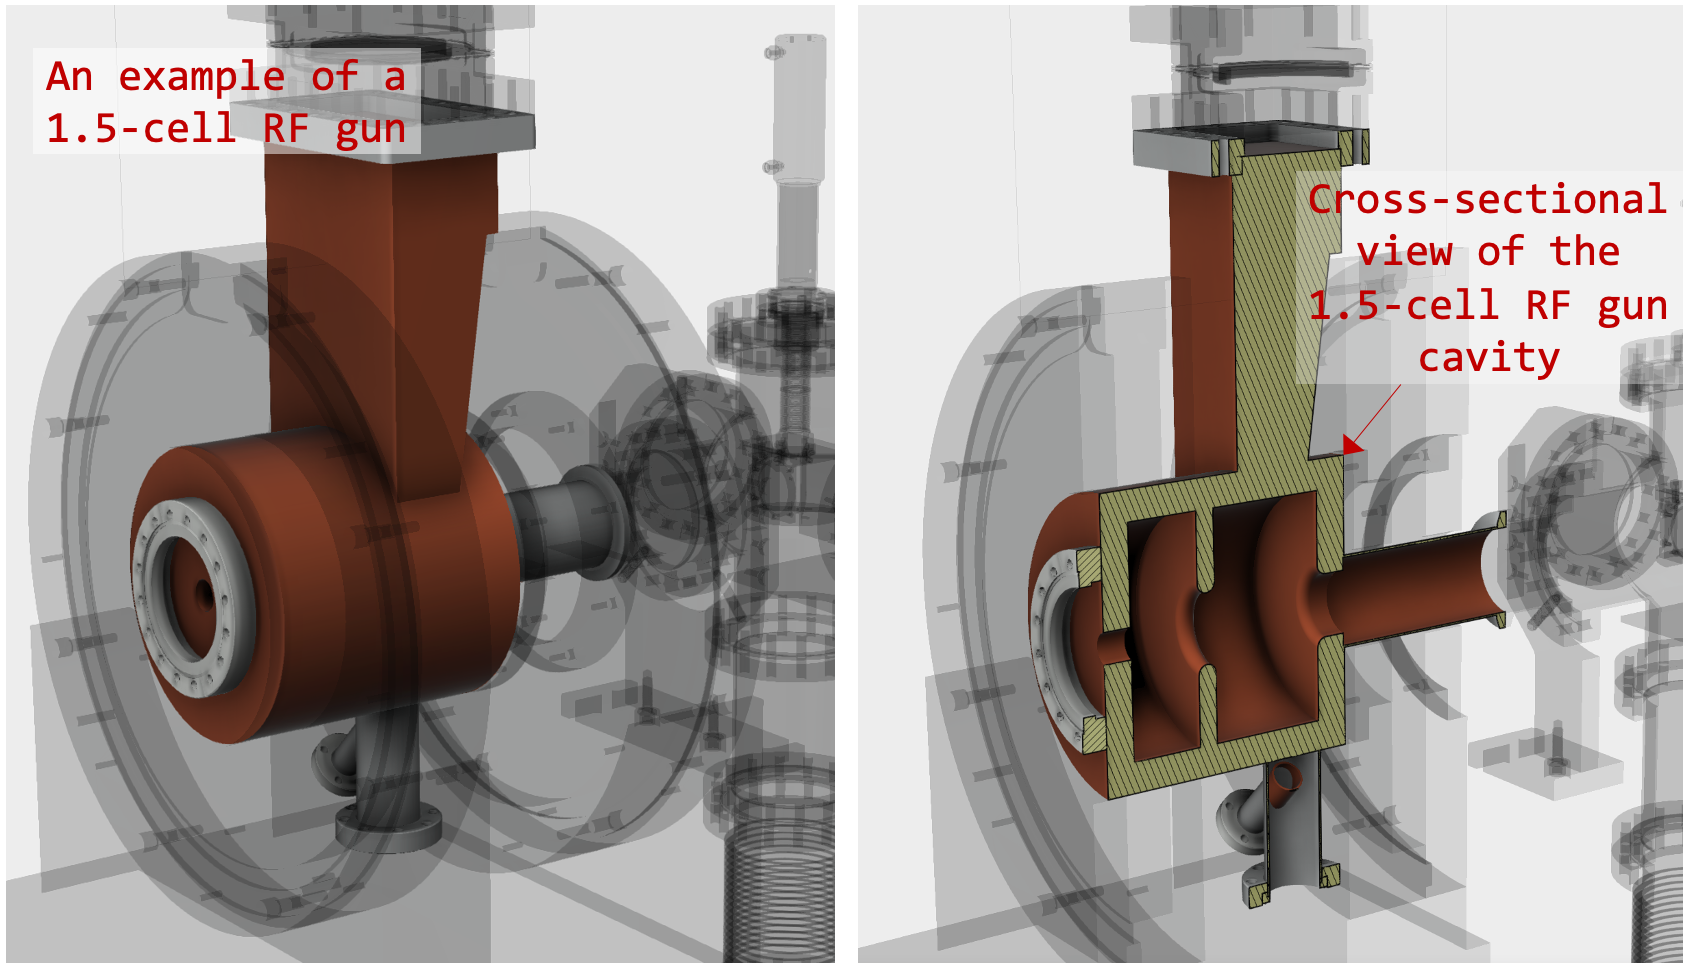
\includegraphics[height=0.6\textwidth]{beamline3_3.png}
    \end{figure}
\end{column}
% Column 2
\begin{column}{0.38\textwidth}
\begin{itemize}
    \item RF gun cavity which generates the \textbf{electromagnetic field} is used to accelerate the electron beams that emitted from the cathode. 
    \item The geometry of the gun needs to be carefully optimized in order to have the desired resonant frequency, Q factor etc.
\end{itemize}
\end{column}
\end{columns}
\end{frame}

\begin{frame}{Introduction to a solenoid magnet}
\begin{columns}
% Column 1 
\begin{column}{0.4\textwidth}
    \begin{figure}
    \centering
        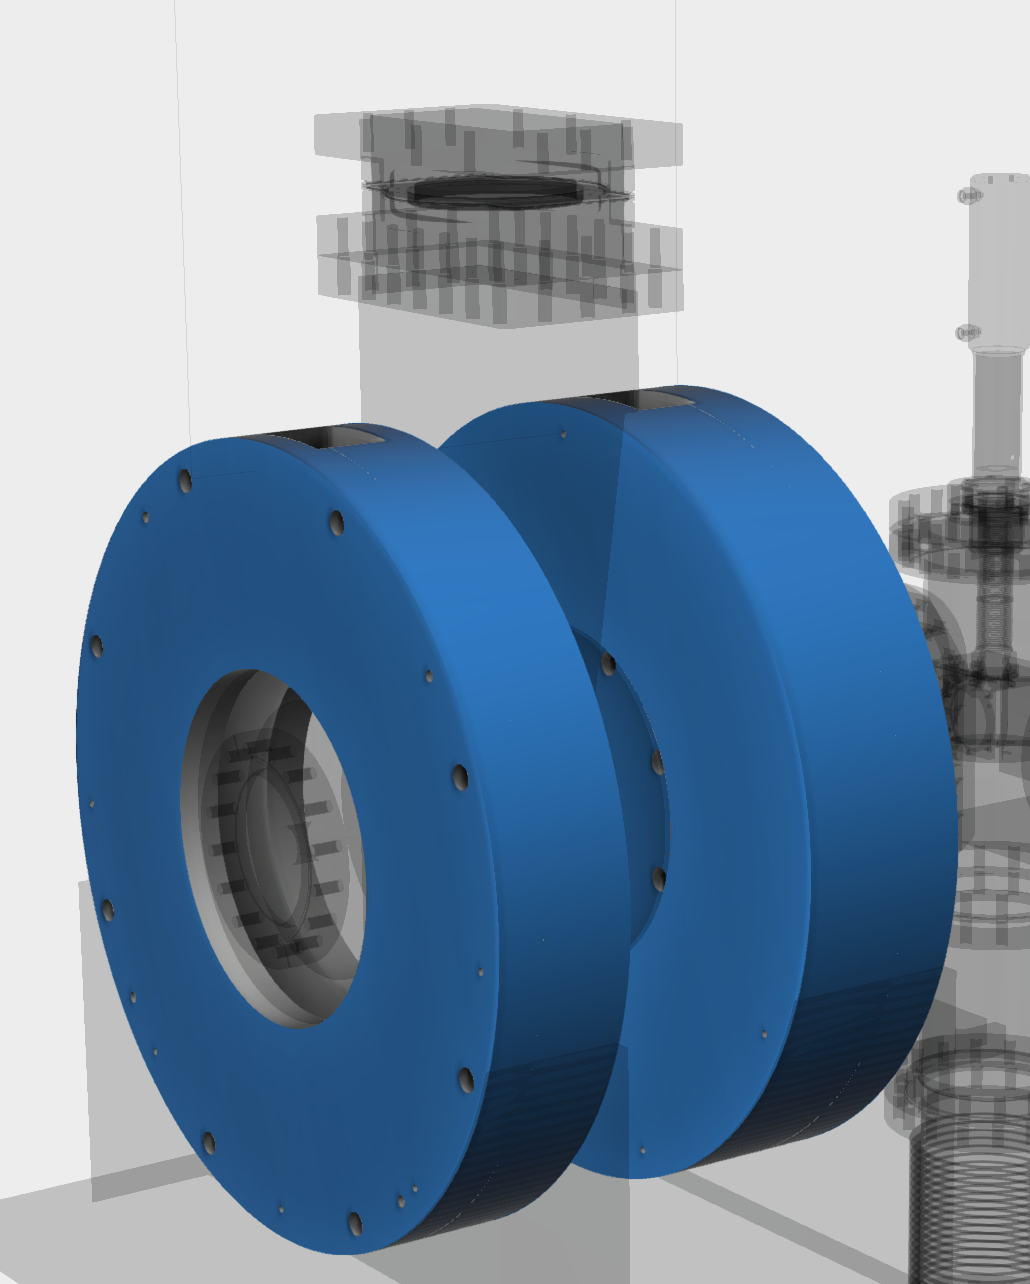
\includegraphics[height=1\textwidth]{beamline4.png}
    \end{figure}
\end{column}
% Column 2
\begin{column}{0.6\textwidth}
\begin{itemize}
\item A solenoid magnet(s) which generates the \textbf{magnetic field} is commonly installed around the RF gun to focus and to confine the transverse emittance ($\varepsilon_{trans}$) of the electron beam. 
\end{itemize}
\end{column}
\end{columns}
\end{frame}

\begin{frame}{Motivation}
\begin{columns}
% Column 1 
\begin{column}{0.6\textwidth}
\textbf{Ultimate Goal} is to produce high brightness beam through the designed beamline (including a RF gun cavity and a main solenoid). 

\textbf{Traditional way} for designing a beamline starts from individual components optimization cavities, magnets and beam dynamics are optimized independently by separate individuals using different codes with isolated targeting objectives, which may not be a direct way of achieving the goal. 

\textbf{Our proposed way} for designing a beamline is by setting up a unified framework by integrating various modules, with the desired objectives (i.e. $\varepsilon_{trans}$, frequency etc.). 
\end{column}
% Column 2
\begin{column}{0.35\textwidth}
\begin{figure}
    \centering
        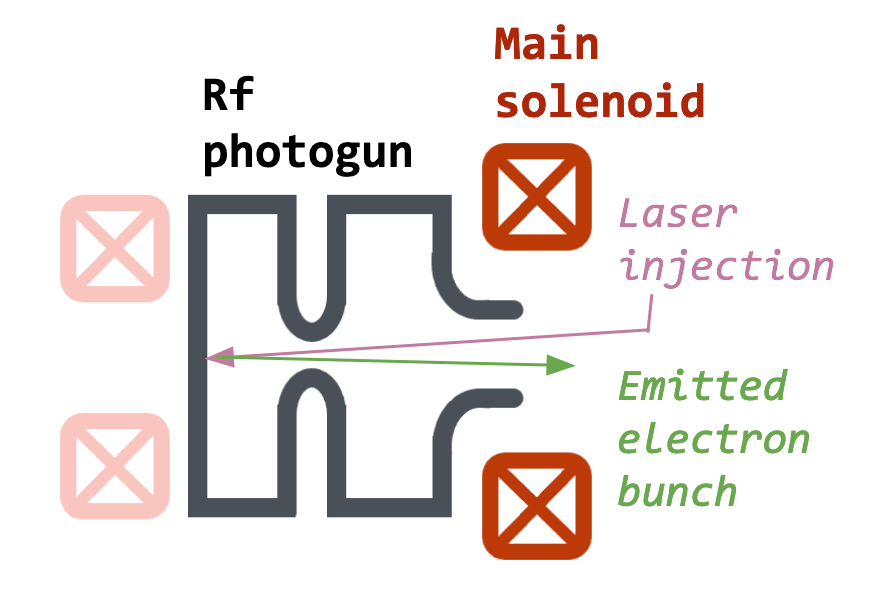
\includegraphics[height=0.7\textwidth]{setup5.png}
    \end{figure}
\end{column}
\end{columns}

\end{frame}

\section{An integrated framework for global optimization}

\begin{frame}{Introduction to the integrated framework}
\begin{center}
        \begin{tikzpicture}
            \node[anchor=south west,inner sep=0] (image) at (0,0) {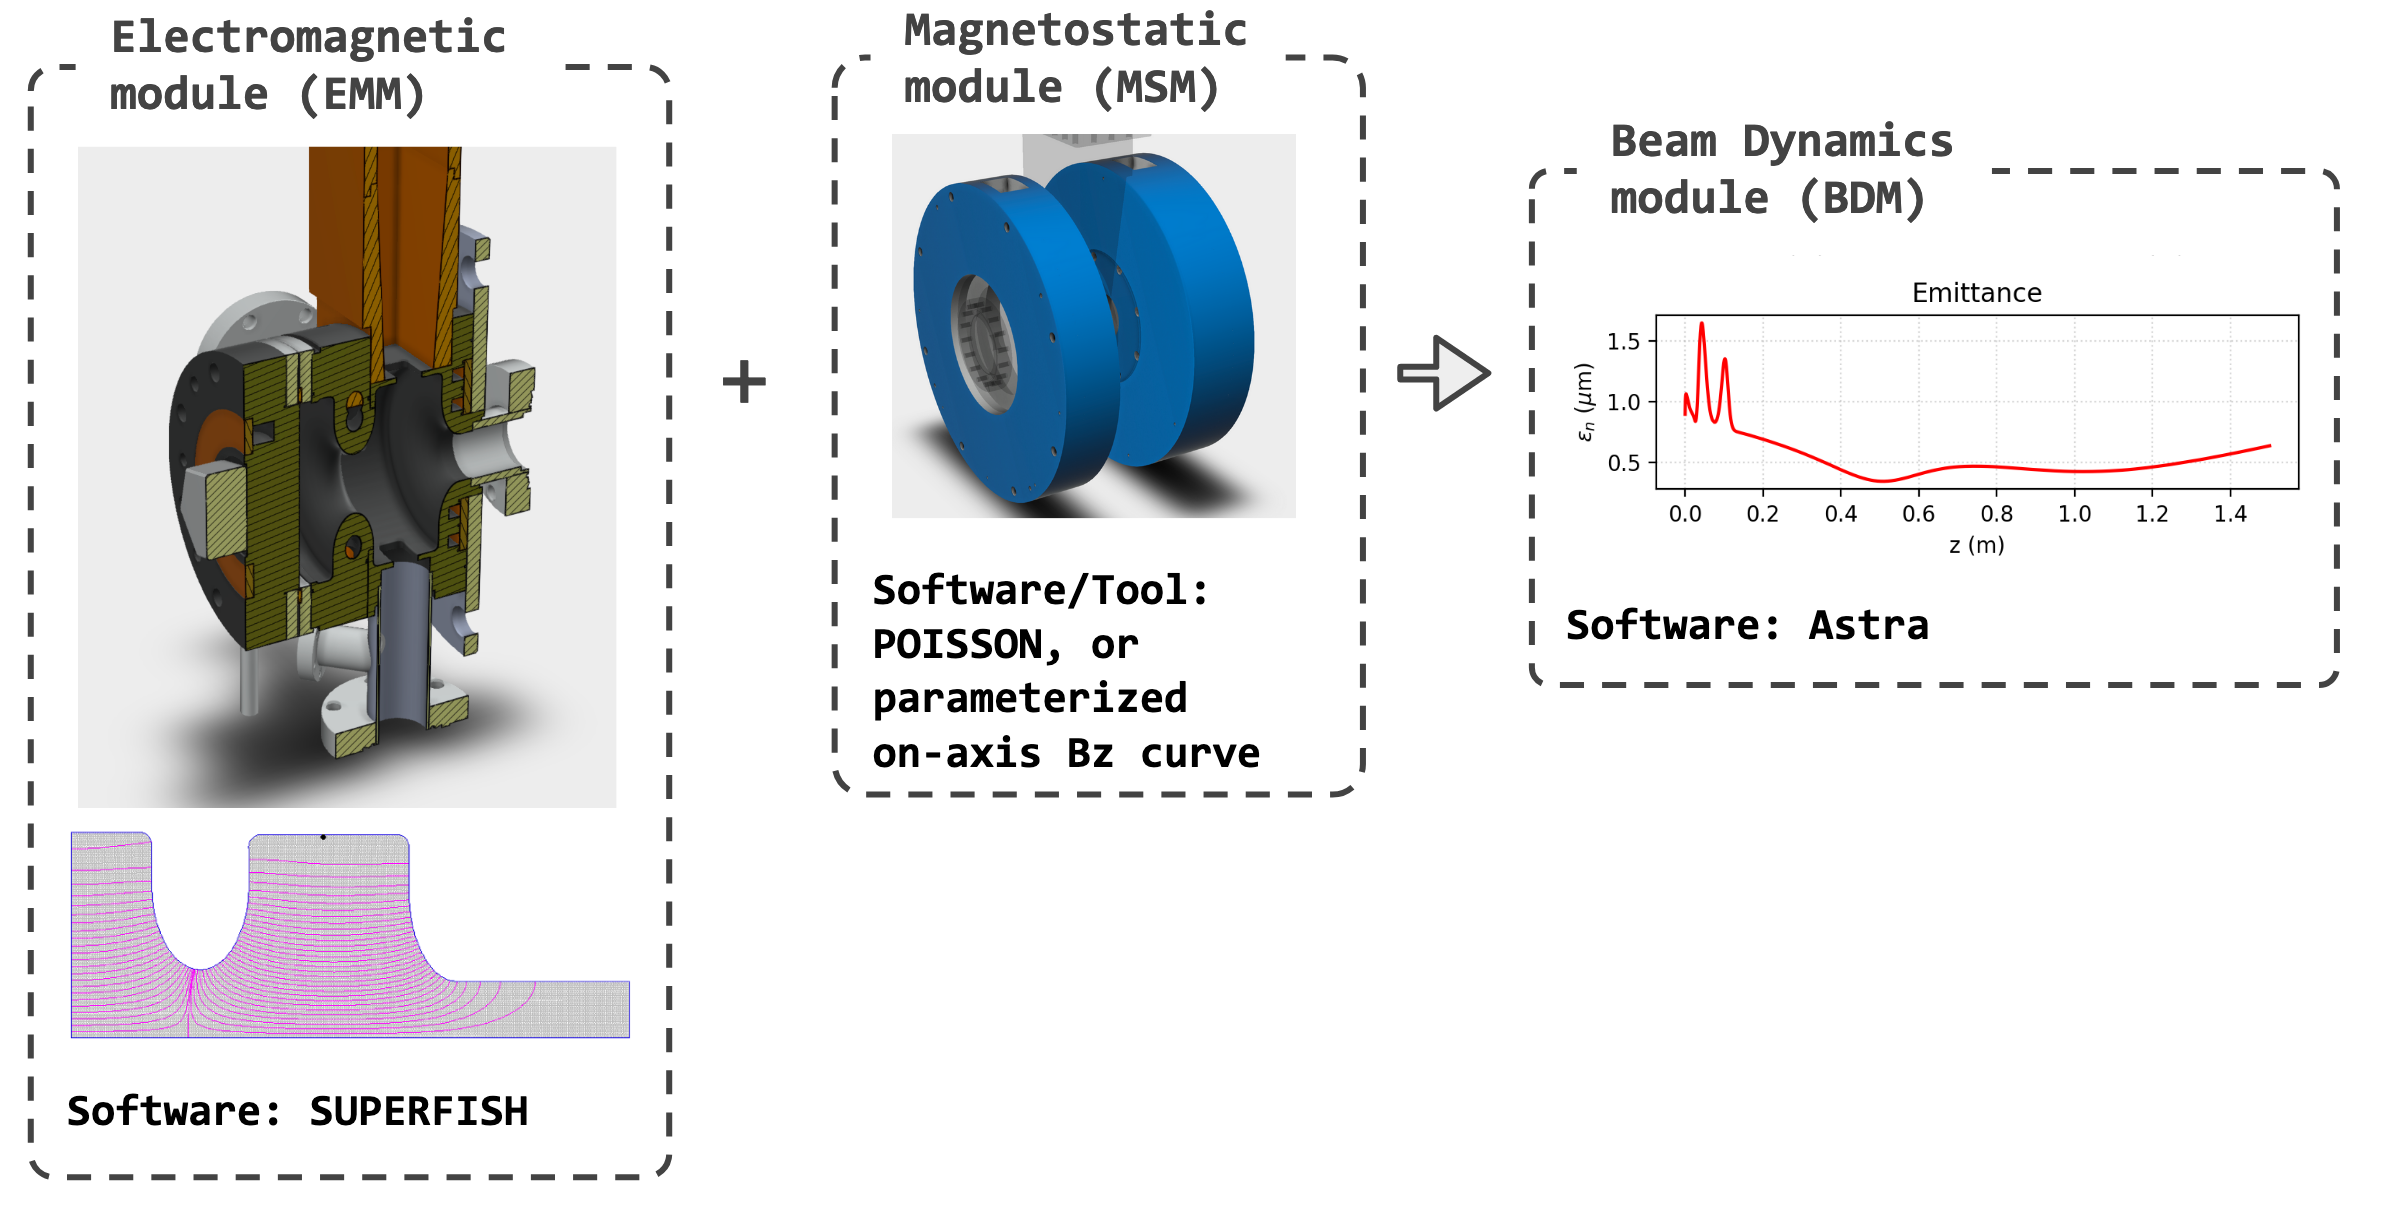
\includegraphics[width=0.9\textwidth]{setup4.png}};
            \node[align=left] at (9, 0.9) {\textbf{Workflow:} the simulated electromagnetic field of the \\optimized gun from EMM and the parameterized on-axis $B_z$\\ from MSM will be used in the BDM for beam dynamics\\ simulations.};
        \end{tikzpicture}
    \end{center}
    
\end{frame}

\begin{frame}{Diagram of Modules}

\begin{center}
        \begin{tikzpicture}
            \node[anchor=south west,inner sep=0] (image) at (0,0) {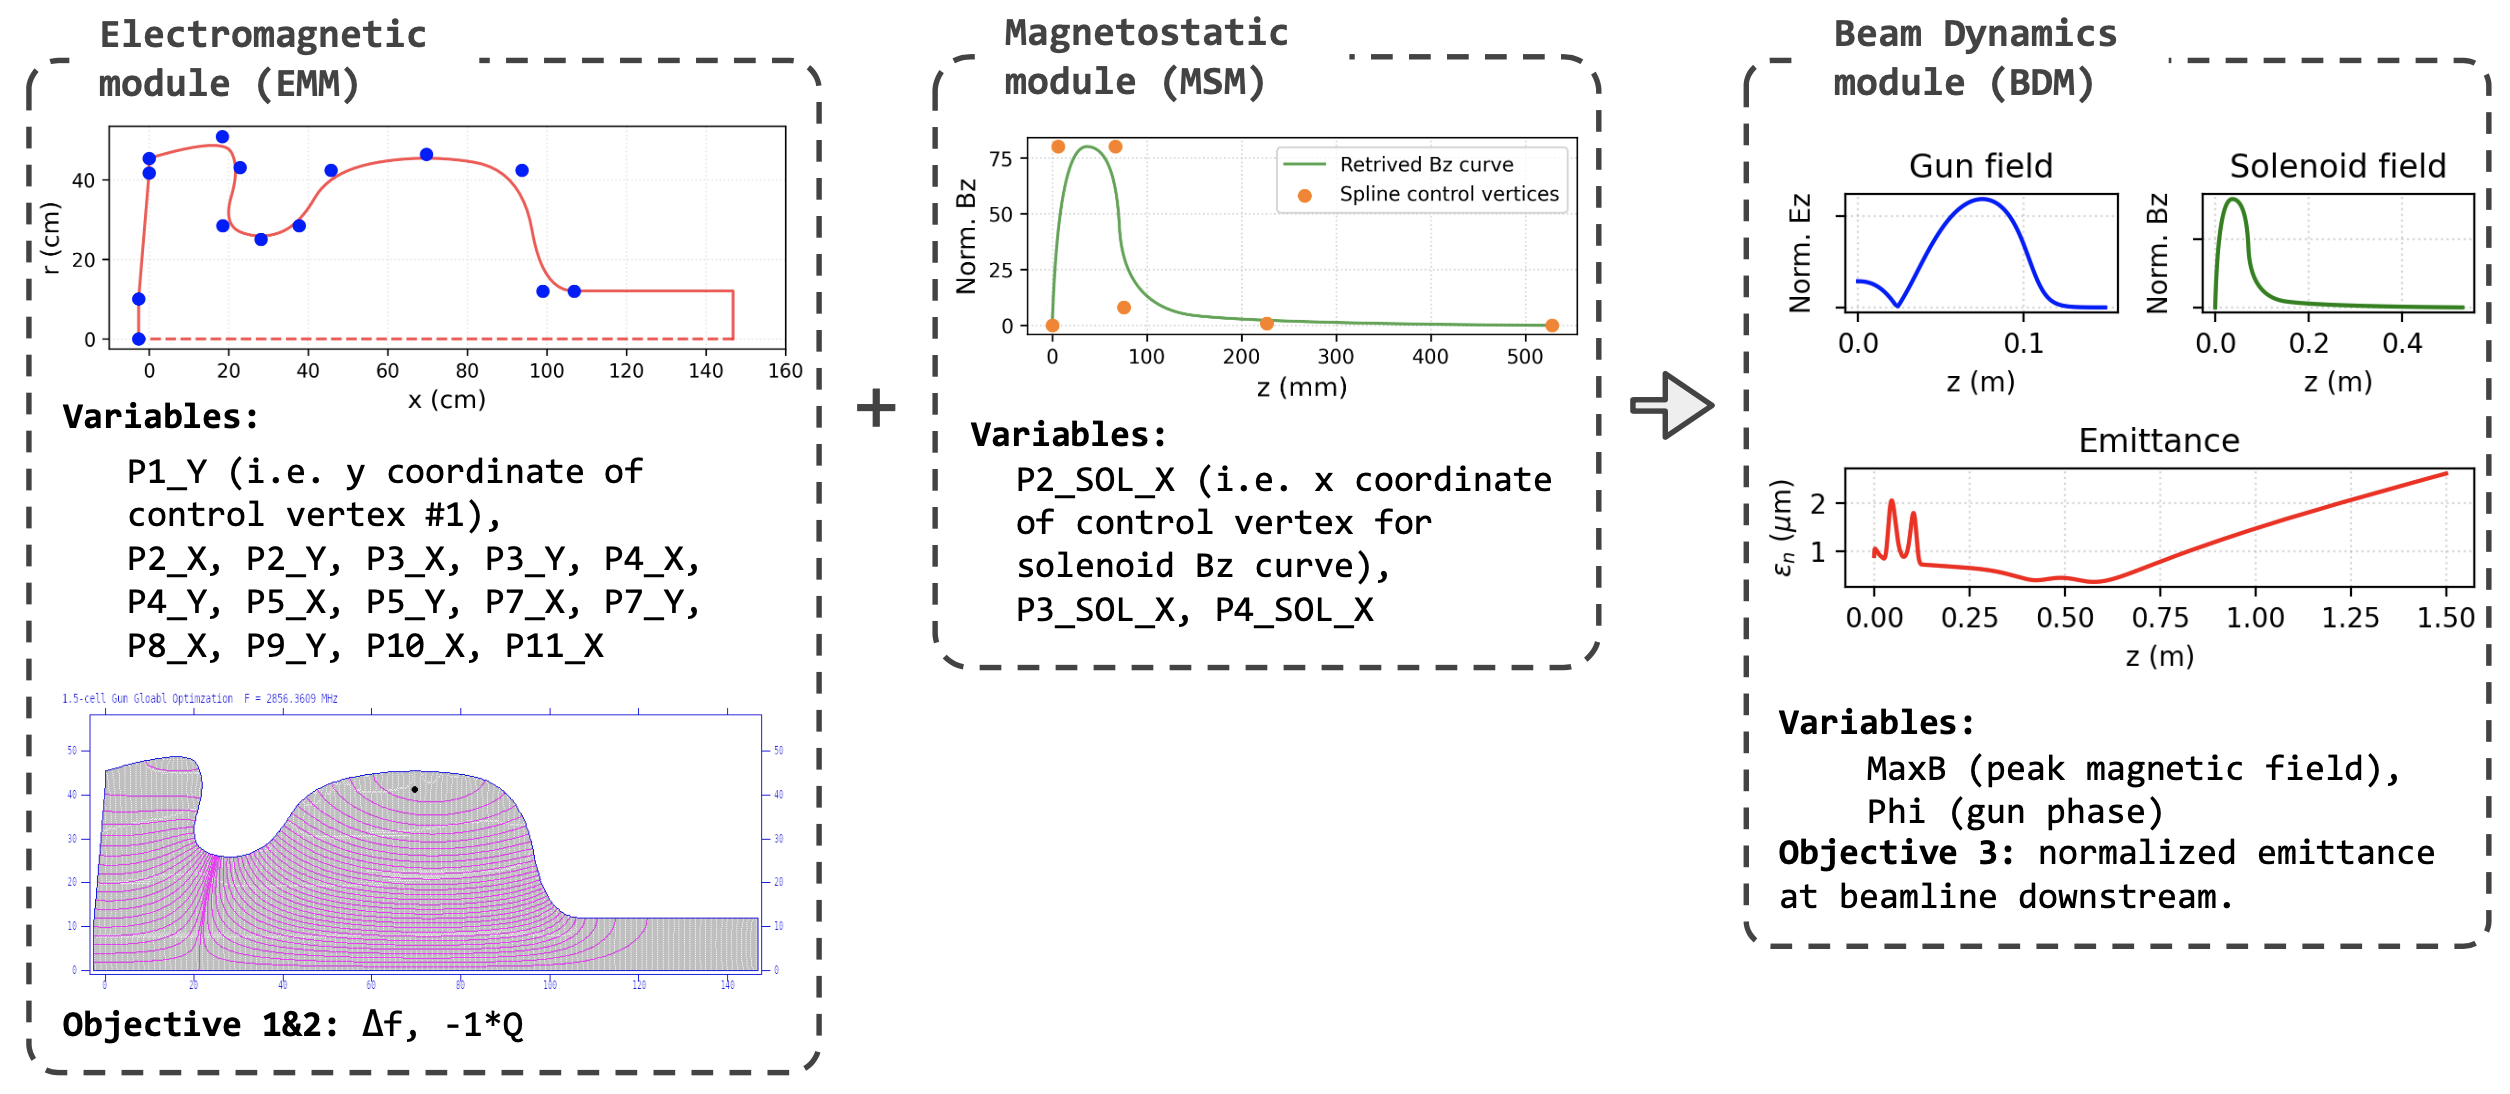
\includegraphics[width=0.9\textwidth]{setup6_2.png}};
            \node[align=left, font=\small] at (6.5, -0.8) {\textbf{Variables in EMM} are coordinates of control vertices to generate the spline (aka.\\ the gun geometry). \textbf{Variables in MMM} are coordinates of control vertices to \\generate the on-axis Bz. \textbf{Variables in BDM} are gun phase and solenoid peak Bz.} ;
        \end{tikzpicture}
    \end{center}
    
\end{frame}

\section{Optimization methods}

\begin{frame}{The Multiobjective Optimization Problem}

    $$
    \min (\text{$\varepsilon_{trans}$ from BDM, -1$\cdot$ Q factor and $\Delta f$ (defined by $\left|f_{target} - f_{simulate}\right|$) from EMM})
    $$

    $$
    \text{for all  MSM shapes, EMM geometries, and BDM settings}
    $$
    
    $$
    \text{ s.t. } \quad \text{few particles lost, beam quality is sufficient, etc.}
    $$
    
\end{frame}

\begin{frame}{The Multiobjective Optimization Problem}

    \centering
    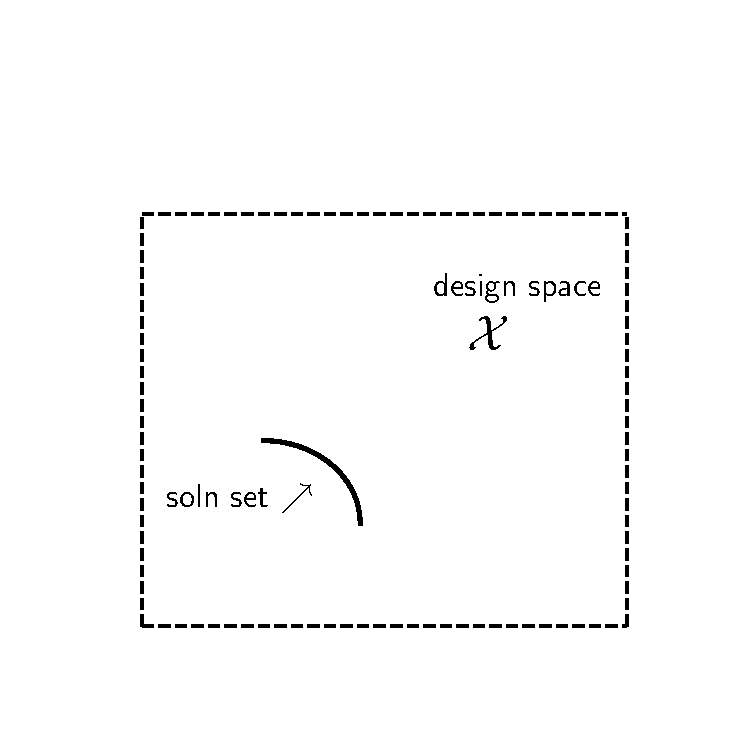
\includegraphics[width=0.45\textwidth]{../img/moo_new/efficient_set-eps-converted-to.pdf}
    $\rightarrow$
    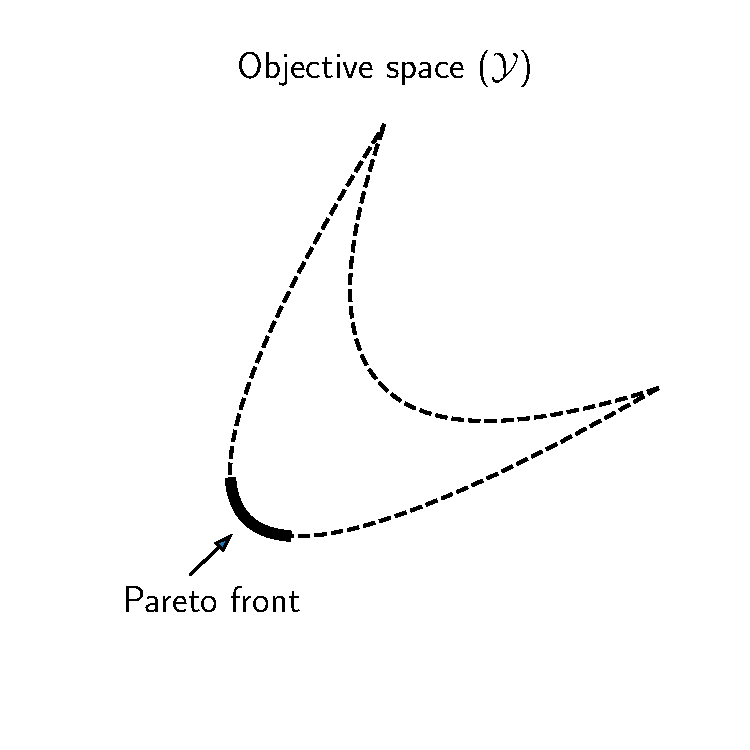
\includegraphics[width=0.35\textwidth]{../img/moo_new/pareto_set-eps-converted-to.pdf}
\end{frame}

\begin{frame}{Optimization Challenges}
    \begin{itemize}
        \item 23 design variables (15 control vertices from EMM + 6 from MSM + 2 from BDM)
        \item Multiple objectives ($\varepsilon_{trans}$, -1$\cdot$ Q factor and $\Delta f$)
        \item For almost all settings, problem is infeasible (particles lost, geometry is not physical, beam quality is poor)
        \item Running all simulations is expensive (10ish minutes on HPC)
        \item No gradients (derivative-free)
    \end{itemize}
    
    \pause 
    \bigskip
    
    {\centering \bf How to tune 23 variables, 3 objectives on limited budget, when almost all settings are infeasible?}
    
\end{frame}

\begin{frame}{Popular Optimization Methodologies}
    \begin{itemize}
        \item Multiobjective Evolutionary/Genetic Algorithms (NSGA-II)
        \item Multiobjective Bayesian Optimization
        \pause \item Multiobjective Trust-region descent?
    \end{itemize}
\end{frame}

\begin{frame}{Scalability of optimization methods}
    \begin{columns}
        \begin{column}{0.49\textwidth}
            \centering
            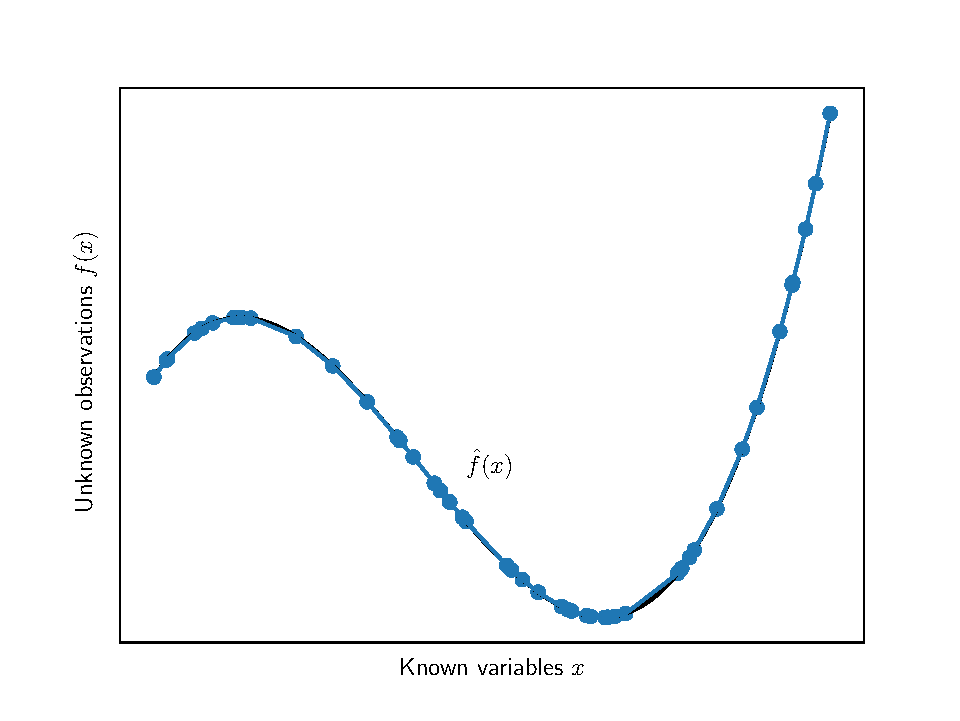
\includegraphics[width=0.75\textwidth]{../img/delaunay_new/inference_1d_pt5-eps-converted-to.pdf}\\
            \onslide<2->{
            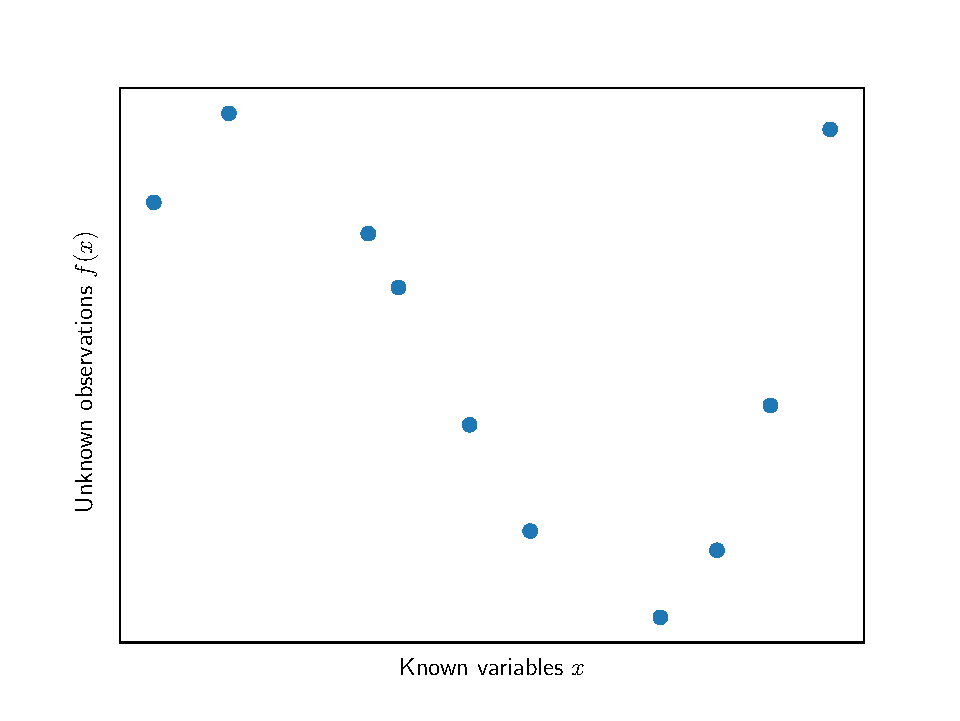
\includegraphics[width=0.75\textwidth]{../img/delaunay_new/inference_2d_pt1-eps-converted-to.pdf}}
        \end{column}
        \begin{column}{0.49\textwidth}
            \centering
            \onslide<3->{
            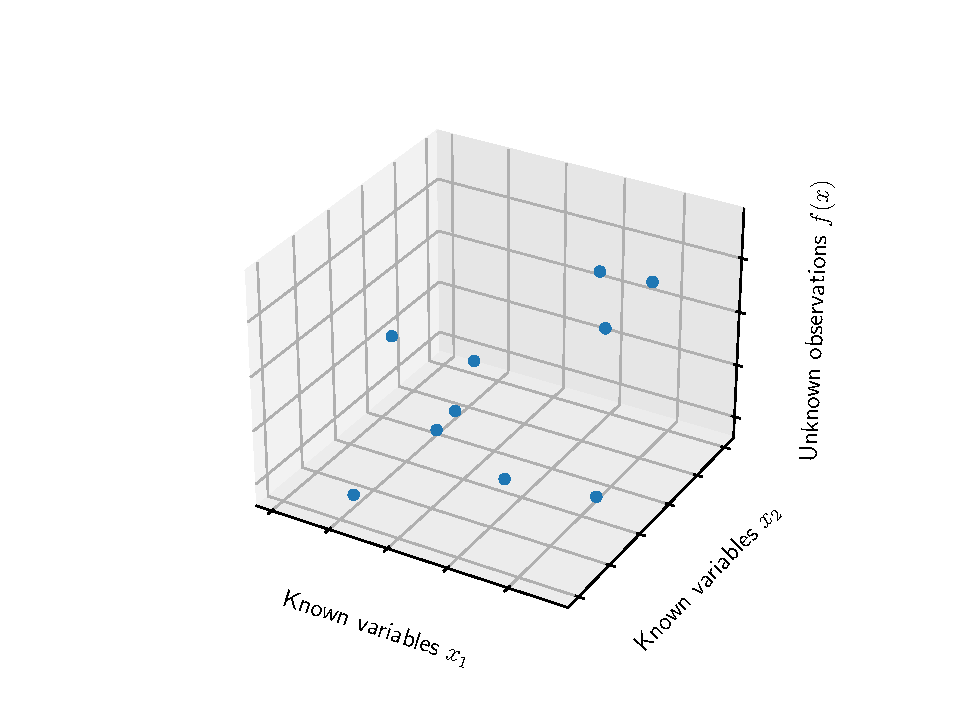
\includegraphics[width=0.75\textwidth]{../img/delaunay_new/inference_2d_pt2-eps-converted-to.pdf}}
            \onslide<4->{
            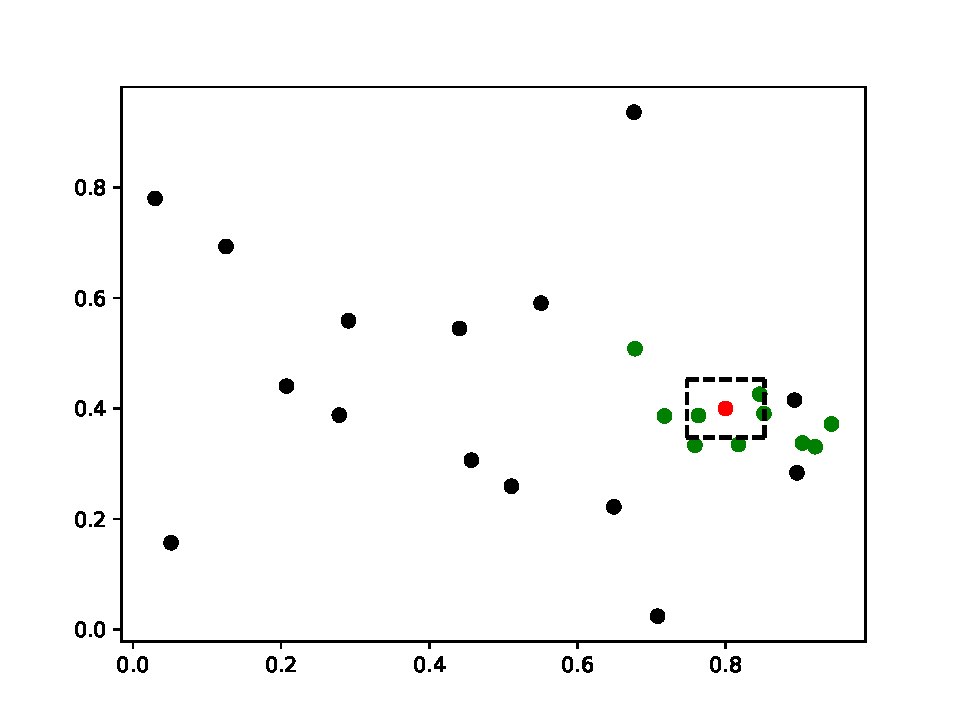
\includegraphics[width=0.75\textwidth]{../img/moo_new/trust_region_pt4-eps-converted-to.pdf}}
        \end{column}
    \end{columns}
\end{frame}

\begin{frame}{Comparison on a test problem}

A 50D, 2 objective, convex test problem, 1000 function evals:

\medskip

Gaussian process surrogate, comparing BO vs.\ Latin hypercube + trust-region

\bigskip

    \begin{columns}
        \begin{column}{0.49\textwidth}
            \centering
            \pause
            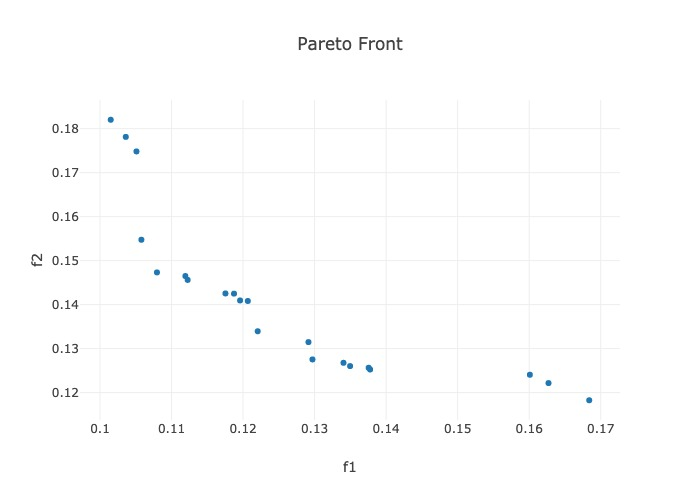
\includegraphics[width=0.8\textwidth]{../img/moo_new/BO_PF.jpeg}\\
            BO
        \end{column}
        \begin{column}{0.49\textwidth}
            \centering
            \pause
            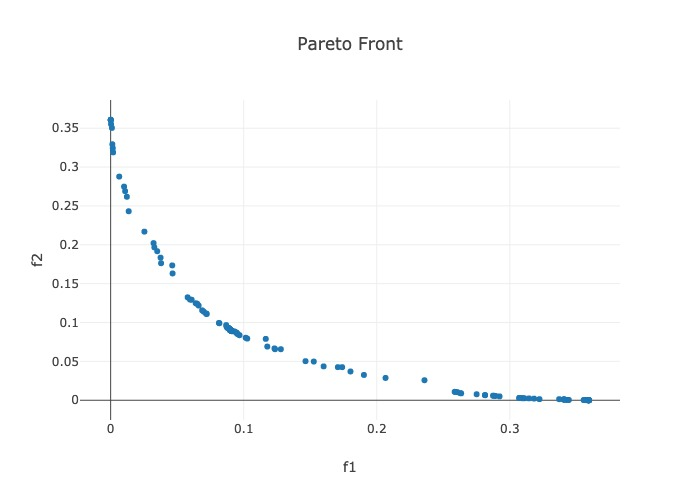
\includegraphics[width=0.8\textwidth]{../img/moo_new/TR_PF.jpeg}\\
            TR
        \end{column}
    \end{columns}

    
\end{frame}

\section{Experiment setup}

\begin{frame}{Software Stack}
\begin{itemize}
    \item EMM + MSM modules: {\tt POISSON/SUPERFISH} -- Fortran SW from 
    \item BDM module: {\tt ASTRA} -- Fortran SW by K. Floetmann (DESY)
    \item Docker image: {\tt github.com/hhslepicka/docker-poisson-superfish-nobin}
    \item Python interface: {\tt github.com/ChristopherMyers/PySuperfish}
    \pause
    \item Optimization SW: {\tt ParMOO} -- Chang \& Wild (ANL)
    \pause
    \item Coordination and workflow on HPC systems: {\tt libEnsemble} -- Hudson, Larson, Navarro \& Wild (ANL)
    \pause
    \item Ran all experiments on the HPC {\tt Bebop} in the LCRC at Argonne
\end{itemize}
\end{frame}

\begin{frame}{Experiment setup}
ParMOO hyperparameters: 

\begin{itemize}
    \item[] \textbf{search budget}: 800 (all infeasible)
    \item[] \textbf{search}: LatinHypercube,
    \item[] \textbf{surrogate}: LocalGaussRBF
    \item[] \textbf{batch size}: 16, where we set 15 randomized scalarizations, and fixed 1 scalarization for emittance optimization.
    \item[] \textbf{total budget}: 5600 over all 300 iterations of localized Gaussian process modeling and trust-region descent.
\end{itemize}
\end{frame}

\begin{frame}{Results of optimization}
\begin{columns}
% Column 1 
\begin{column}{0.6\textwidth}
\begin{itemize}
    \item Given a initial beam source with rms spot size ($\sigma_x$) of 0.5~mm, bunch length (FWHM) of 300~fs, bunch charge of 100~pC, along with a standard operation gun gradient of 150~MV/m.
    \item The emittance generated by the optimized beamline was found to converge to <0.3~$\mu$m, which is comparable to state-of-the-art results. An example of the optimized result is shown here.
    \item Solution was found within the first 2000 function evaluations.
\end{itemize}

\end{column}
% Column 2
\begin{column}{0.4\textwidth}
\begin{figure}
    \centering
        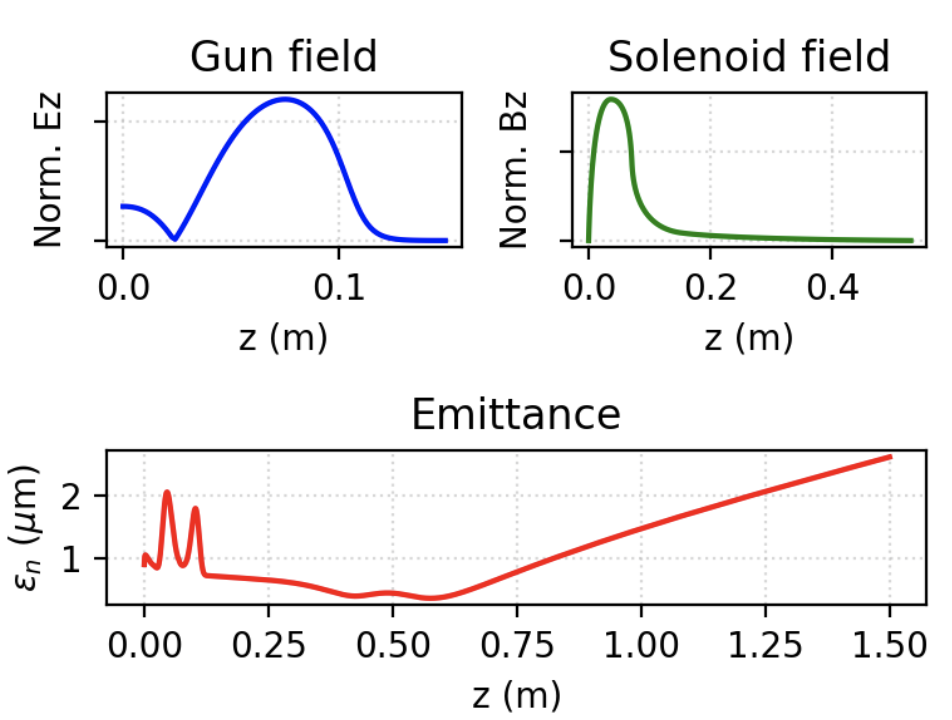
\includegraphics[height=0.7\textwidth]{optm1.png}
    \end{figure}
\end{column}
\end{columns}
\end{frame}

\section{Conclusion and Future Work}

\begin{frame}{Conclusions and future work}

{\bf Conclusion of this Study:}

\begin{itemize}
    \item Our proposed platform by integrating multi-physics modules shows significant efficiency in the design of rf structures.
    \item With the unified platform, a new Linac cavity has been proposed and designed.
    \item Our optimization methods are able to tune these complex geometries for multiple obejctives on a realistic budget.
\end{itemize}


\bigskip
\pause {\bf Next Steps:}

\begin{itemize}
    \item Perform more rigorous experiments and comparisons with other optimization methods and previous works.
    \item Explore the tuning of other aspects of geometry such as cell lengths and additional concave features.
\end{itemize}
\end{frame}

\begin{frame}\frametitle{Acknowledgments}
\vfill 

This work is supported by Laboratory Directed Research and Development (LDRD) funding from Argonne National Laboratory.

\medskip

This work was also supported in part by the U.S.~Department of Energy, Office of
Science, Office of Advanced Scientific Computing Research and Office of
High-Energy Physics, Scientific Discovery through Advanced Computing (SciDAC)
Program through the FASTMath Institute and the CAMPA Project under Contract
No.~DE-AC02-06CH11357.

\medskip

We gratefully acknowledge the computing resources provided on Bebop, a HPC cluster operated by the Laboratory Computing Resource Center at Argonne National Laboratory.

\medskip

We thank Philippe Piot for the insightful discussions on the simulations.
We also thank Jeff Larson, John-Luke Navarro, and Steve Hudson for their advice on libEnsemble usage.

\end{frame}

\end{document}


